% --- chapter
\newcommand{\chapter}[2][]{
	\newcommand{\chapname}{#2}
	\begin{flushleft}
		\begin{minipage}[t]{\linewidth}
			
\includegraphics[height=1cm]{hdht-logo.png}
			\hspace{0pt}	
			\sffamily\bfseries\large Bài  23. Nguyên tắc thông tin liên lạc bằng sóng vô tuyến
			\begin{flushleft}
				\huge\bfseries #1
			\end{flushleft}
		\end{minipage}
	\end{flushleft}
	\vspace{1cm}
	\normalfont\normalsize
}
%-----------------------------------------------------
\chapter[Nguyên tắc thông tin liên lạc\\ bằng sóng vô tuyến]{Nguyên tắc thông tin liên lạc bằng sóng vô tuyến}

	\subsection {Nguyên tắc chung của việc thông tin liên lạc bằng sóng vô tuyến}
\begin{itemize}
	\item Dùng sóng điện từ cao tần.
	\item Biến điệu sóng mang.
	\item Tách sóng.
	\item Khuếch đại.
\end{itemize}
\subsection {Sơ đồ khối của máy phát thanh vô tuyến đơn giản}
\begin{center}
	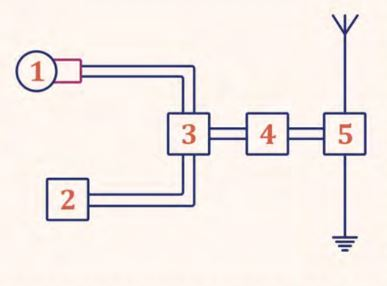
\includegraphics[scale=0.5]{../figs/4-4-1.JPG}
\end{center}
\begin{enumerate}
	\item \bltext{Micrô.}
	\item \bltext{Mạch tách sóng điện từ cao tần.}
	\item \bltext{ Mạch biến điệu (trộn sóng điện từ).}
	\item \bltext{ Mạch khuếch đại.}
	\item  \bltext{Anten phát.}
\end{enumerate}
\subsection {Sơ đồ khối của một máy thu thanh vô tuyến đơn giản}
\begin{center}
	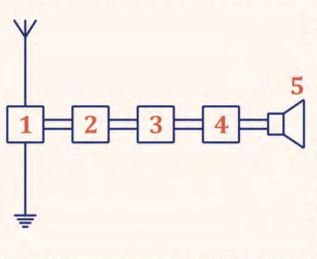
\includegraphics[scale=0.7]{../figs/4-4-2.JPG}
\end{center}
\begin{enumerate}
	\item \bltext{Anten thu.}
	\item \bltext{Mạch khuếch đại điện từ cao tần.}
	\item \bltext{Mạch tách sóng.}
	\item \bltext{Mạch khuếch đại dao động điện từ âm tần.}
	\item \bltext{Loa.}
\end{enumerate}
\subsection {Ứng dụng của sóng điện từ}
Sóng vô tuyến điện dùng để tải các thông tin, âm thanh và hình ảnh. Nhờ đó con người có thể thông tin liên lạc từ vị trí này đến vị trí khác trên mặt đất và trong không gian mà không cần dây dẫn.